\documentclass[12pt, letterpaper]{article}
\usepackage[margin=0.8in]{geometry}
\usepackage[utf8]{inputenc}
\usepackage[super,comma]{natbib}
\usepackage{graphicx}
\usepackage{xcolor}

\title{CMSC499A: Mutation Visualization}
\author{Mark Keller \thanks{mentored by Professor Max Leiserson}}
\date{Spring 2018}

\begin{document}
\maketitle

\begin{abstract}
Identification and analysis of patterns in data can be difficult without visualization tools. 
Datasets of somatic mutations in cancer are no exception.
Recent whole-genome sequencing projects have produced large amounts of mutation data to be explored.
Of great importance is the classification of different mutational processes and the mutational signatures\cite{alexandrov2013signatures} they leave behind.
As new mutational signatures continue to be discovered, observation of the levels of signature activity, called signature exposure, helps show how the underlying mutational processes differ across cancer types, time, and environmental variables.
This paper describes a mutation visualization tool developed this semester that allows simple somatic mutation datasets and mutation signatures to be explored interactively and provides users with publication-ready graphics.
\end{abstract}

\section{Introduction}
Slight modifications to data sources used in past studies of mutations and mutation signatures have the potential to solidify or weaken conclusions made based on limited data.
For example, one might be interested in reproducing a past study across additional cancer types or in the context of additional variables, such as smoking status or age.
Web-based interactive visualizations allow for this type of comparison to be done across datasets and features in a way that is accessible and fast.
This semester, I have focused on building a visualization tool to do just this, using whole-genome simple somatic mutation datasets, donor clinical datasets, and mutation signature definitions from various sources.

The resulting tool, located at https://link.lrgr.io, is a web-based mutation data browser that enables exploration of mutational signatures, single-nucleotide variant (SNV) mutation types, and mutation density.
It allows users to choose sequencing project datasets by cancer type, as well as mutational signature combinations (of which can be selected based on cancer-type-specific presets) before plotting this data. 
The following are types of plots that can be generated:
\begin{enumerate}
\item To illustrate estimated contributions of a selected combination of mutational signatures, a stacked bar plot can be generated, showing estimated signature exposures for a sample, along with tobacco and alcohol usage indicators.
    Exposure values can be normalized to sum to one for each sample, or kept relative to the total number of mutations in each sample.
    This plot type was inspired by Figure 4 in Kim \textit{et al.} 2016 that displays estimated contributions of 4 different signatures and tobacco usage over cohorts of urothelial cancer tumor samples \cite{kim2016somatic}.
    
\item To identify samples containing instances of localized hypermutation, called kataegis, this second type of plot highlights kataegis events along the genome.
    Along the vertical axis are samples, and along the horizontal axis is the genome.
    Users can zoom and pan along each chromosome, and easily pinpoint kataegis events by the dark bars located on mutations in kataegis regions.
    Samples are grouped by sequencing project and cancer type.
    This plot doubles as a rainfall plot selector, as each sample bar can be clicked to generate a corresponding rainfall plot.
    To our knowledge, this style of plot has not been used before to visualize kataegis events.
    
\item To examine mutation clusters, specifically those occurring in kataegis regions, a rainfall plot can be generated for each sample.
    Mutations are plotted horizontally based on their genome location, and vertically by the distance (in bp) to the previous mutation.
    Rainfall plots are commonly used to examine regions of hypermutation, as they allow these regions to be easily identified by vertical ``thunderbolts" of mutations. 
    This terminology is related to the name ``kataegis", which is derived from the Greek word for ``thunder".
    Similar rainfall plots can be seen in Figure 4 of Nik-Zainal \textit{et al.} 2012\cite{nik2012mutational}.
    
\item Mutation signature activity across the genome can be explored with a manhattan plot that assigns signatures to individual mutations and groups mutations into bins by chromosome location and signature.
    A signature is assigned to each mutation category (left flanking base pair, single-nucleotide variant, right flanking base pair) for each sample by first computing estimated signature exposures for a sample, then taking the maximum of the product of each signature's probability for the mutation category and the sample's exposure to the same signature.
    These assignments are used to group mutations into bins representing the number of mutations for each signature and genomic region.
    To our knowledge, this is a new method and plot type for exploring signature exposures along the genome.

\end{enumerate}

\begin{figure}
    \caption{Screenshot}
    \centering
    \frame{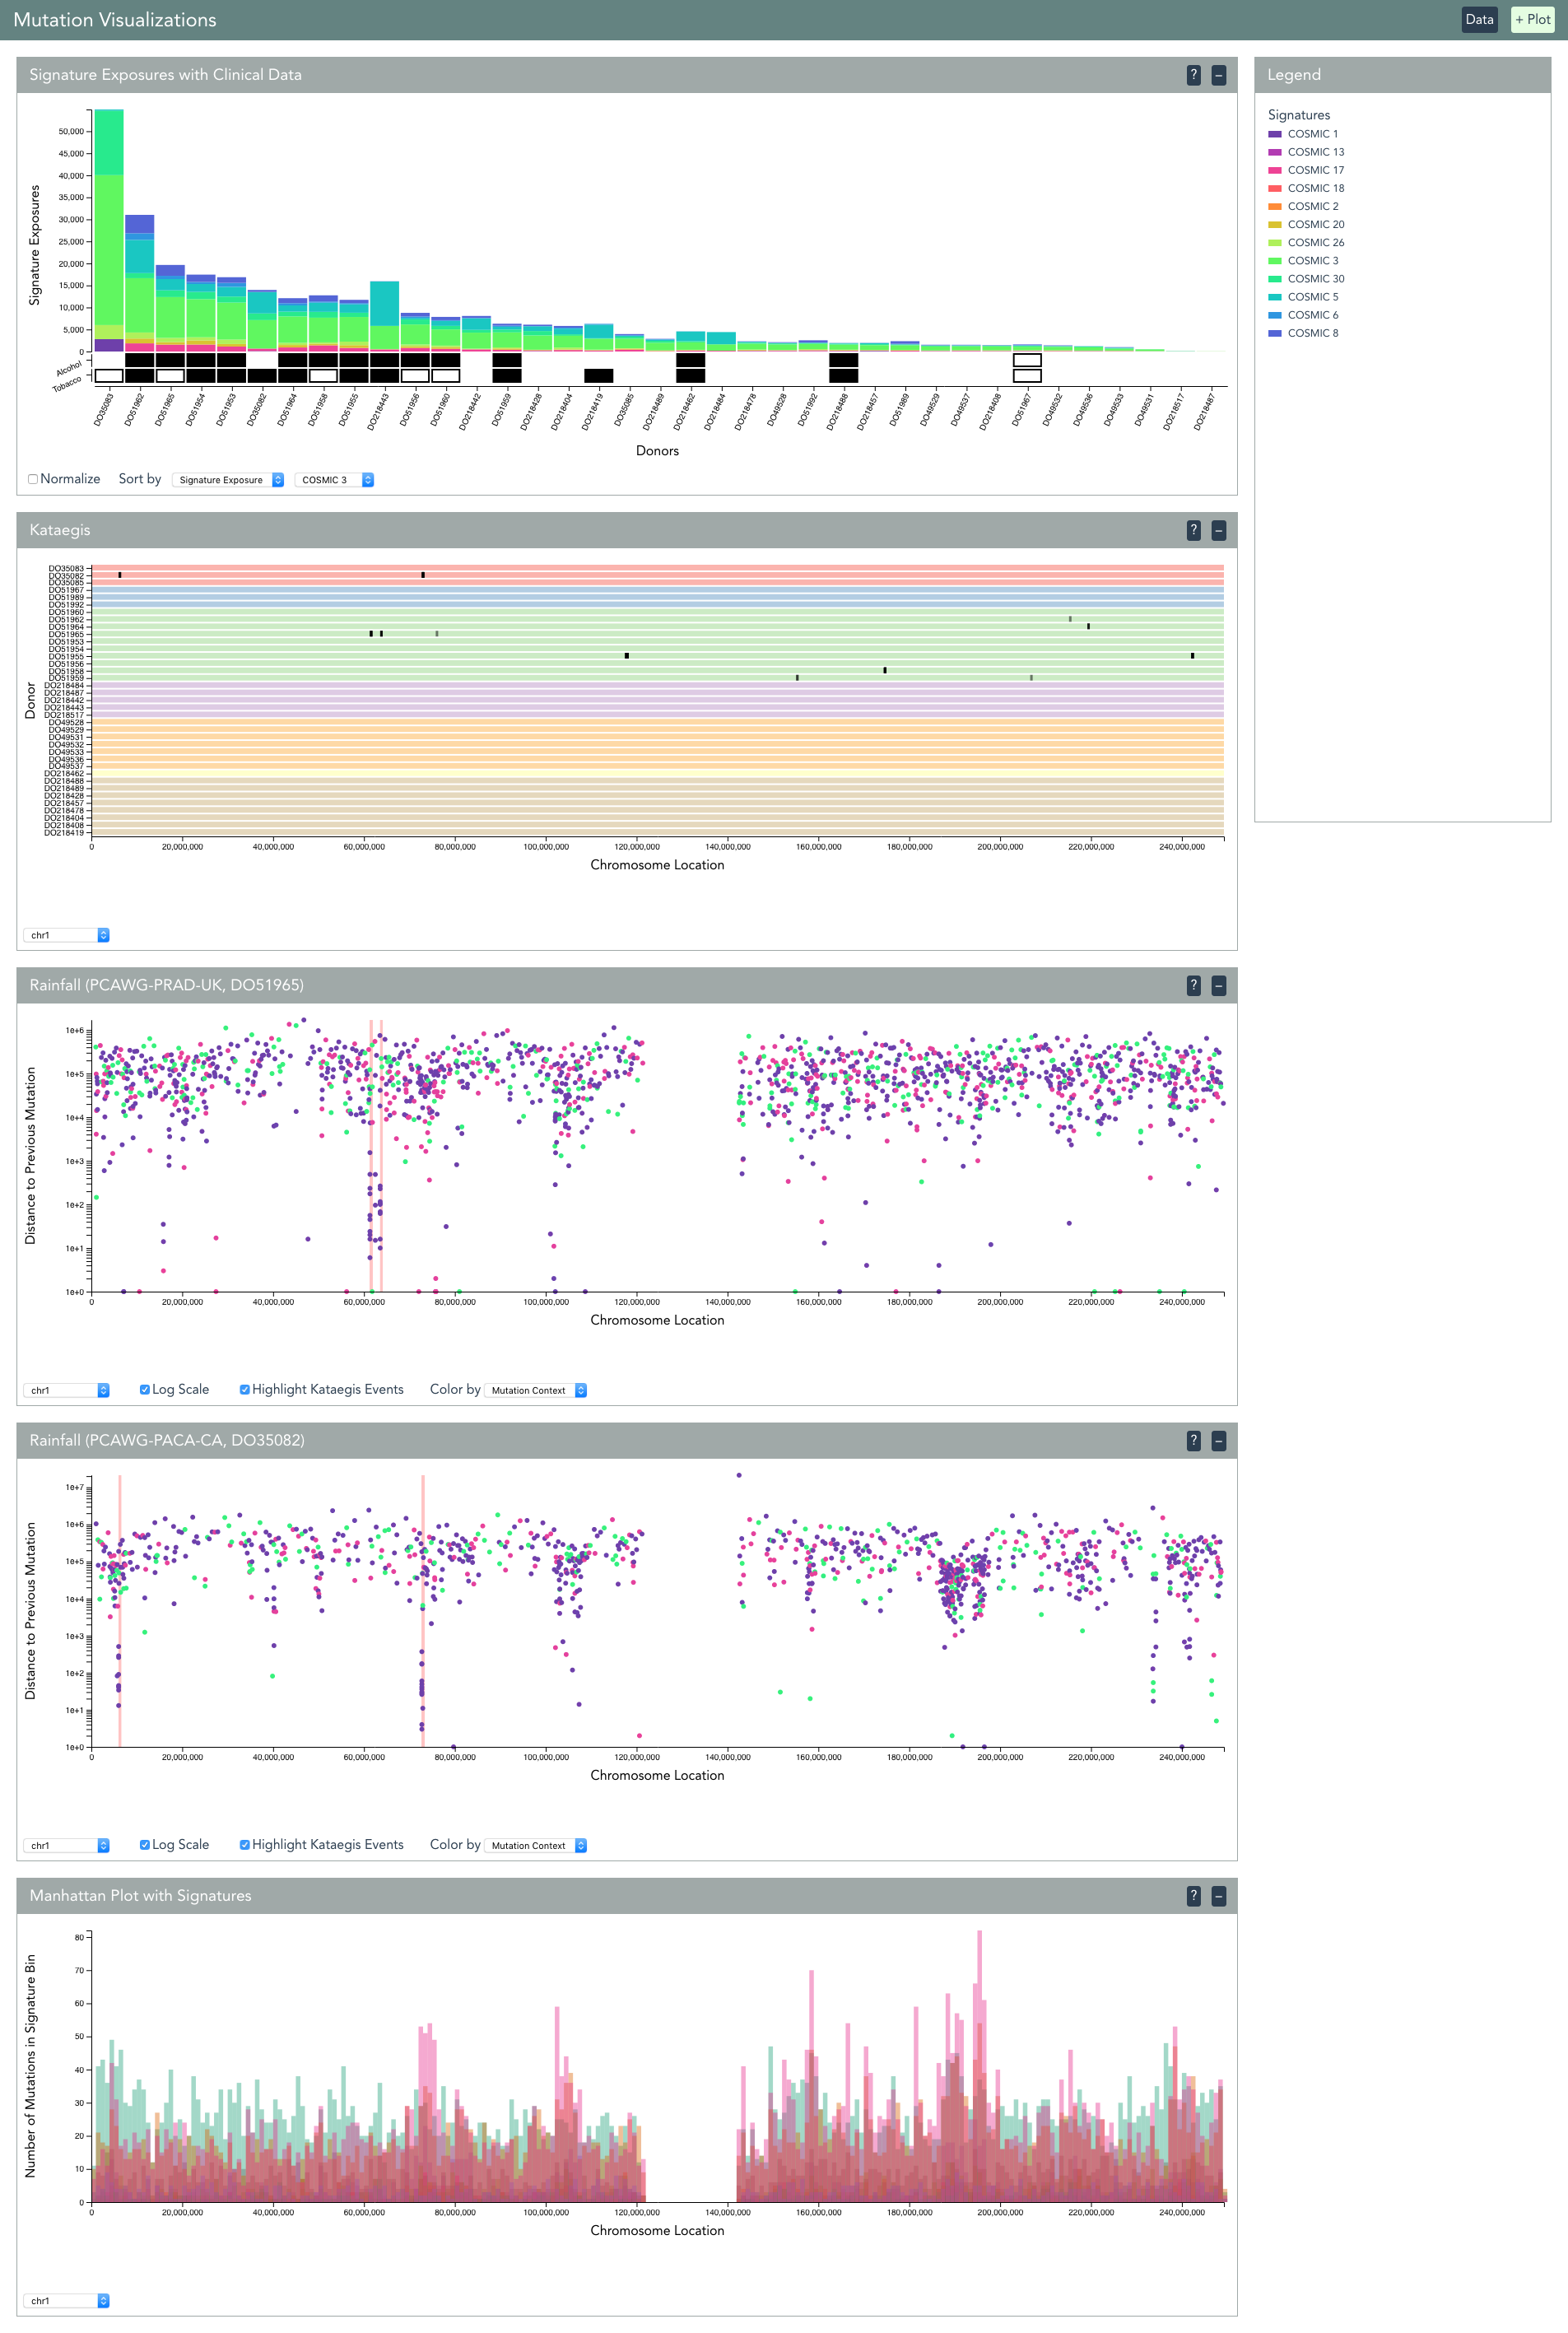
\includegraphics[width=0.8\columnwidth]{figures/screenshot1.png}}
\end{figure}


\section{Case Study}
A potential use case for this tool is the analysis of relationships between signature exposures and clinical variables.
Interactive sorting and dynamic calculations of signature exposures allow trends to be observed quickly.
Connections generally assumed to exist can be verified and examined, such as specific signatures being associated with tobacco usage.

\subsection{Tobacco Usage and Mutational Signatures}
Alexandrov \textit{et al}. 2016 finds that smokers exhibit increases in mutations attributed to COSMIC signatures 2, 4, 5, 13, and 16 \cite{alexandrov2016mutational}. 
Signature 4 in particular ...

\subsection{Tobacco Usage and Hypermutation}

% TODO: Mention sharing with URL


\section{Methods}
Using the data-driven documents JavaScript library (D3.js)\cite{bostock2011d3}, each type of plot is tailored to suit the data types and data sets presented.
Showing donor clinical variables, such as smoking and alcohol usage, and their relationship to mutation signatures, requires this fine control that D3 provides.
In addition, D3 contains APIs for easy implementation of custom interactive features, such as highlighting, panning, and zooming.
Interactivity extends beyond single plots, linking plots together based on variables such as chromosome region and donor ID.

% TODO: Further discussion of plot linking 

This tool has been developed with maintainability and modularity in mind.
Using the Vue JavaScript framework, the application is made up of reusable components that encapsulate templates, functions, and variables.
Component state can be linked to events or ``watchers'' that observe and process data automatically upon change.
This functionality allows data to be bound to page elements or inputs easily.

Data processing occurs in two stages. 
Simple somatic mutation datasets and donor clinical datasets from sequencing projects are downloaded and processed into a uniform format. 
This conversion must be specified for each sequencing project, as each provides datasets in a different format.
Once into a uniform format, these datasets can be processed dynamically by a web server as specific requests are made for visualizations.
This dynamic processing is performed by a web application written in Python with the Flask framework. 
The Pandas and NumPy packages are used for data manipulation in both of these processing stages.

Signature exposures are estimated using a quadratic programming approach detailed by Huang \textit{et al}. 2017\cite{huang2017detecting}.
Signatures present in each cancer type, or signature combination ``presets", are based on those specified in publications of mutational signatures.
For example, the COSMIC signature presences can be found in Figure 3 of Alexandrov \textit{et al}. 2013\cite{alexandrov2013signatures}.

While this software can be run locally, accessing a hosted version may be easier for some users.
Currently, an instance of the Flask-powered web server is deployed to Heroku.
An instance of the front end (Vue/D3) component is deployed through GitHub pages, and uses Travis CI for continuous integration and deployment.
This makes access and usage as simple as connecting via a web browser.

\section{Future Directions}
% TODO
%Local datasets can be visualized, allowing functionality to extend beyond the public datasets we have processed.


\bibliography{main}{}
\bibliographystyle{plain}

\pagebreak
\appendix                                     
\section{Examples of Publication-Ready Figures}
\renewcommand{\figurename}{Example Figure}
\setcounter{figure}{0}

\begin{figure}[h!]
    \caption{Signature Exposures with Clinical Variables}
    \centering
    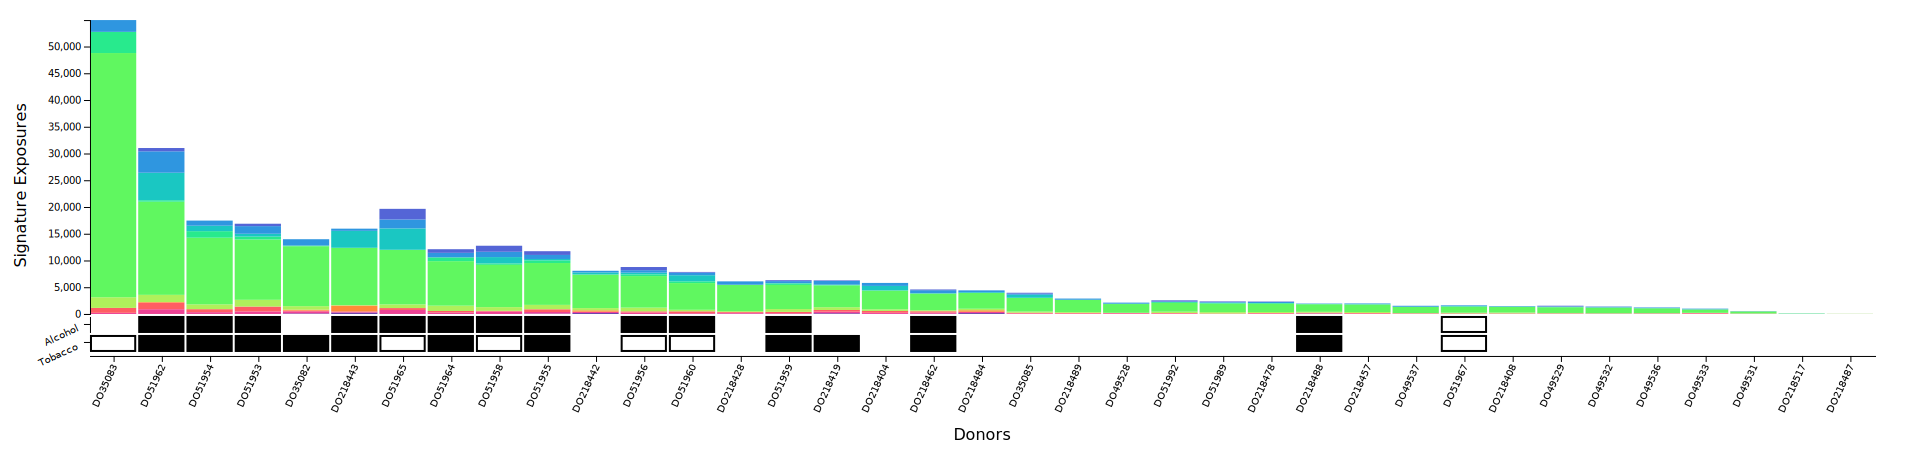
\includegraphics[width=\columnwidth]{figures/exposures.pdf}
\end{figure}
\begin{figure}[h!]
    \caption{Kataegis Plot (Chromosome 2)}
    \centering
    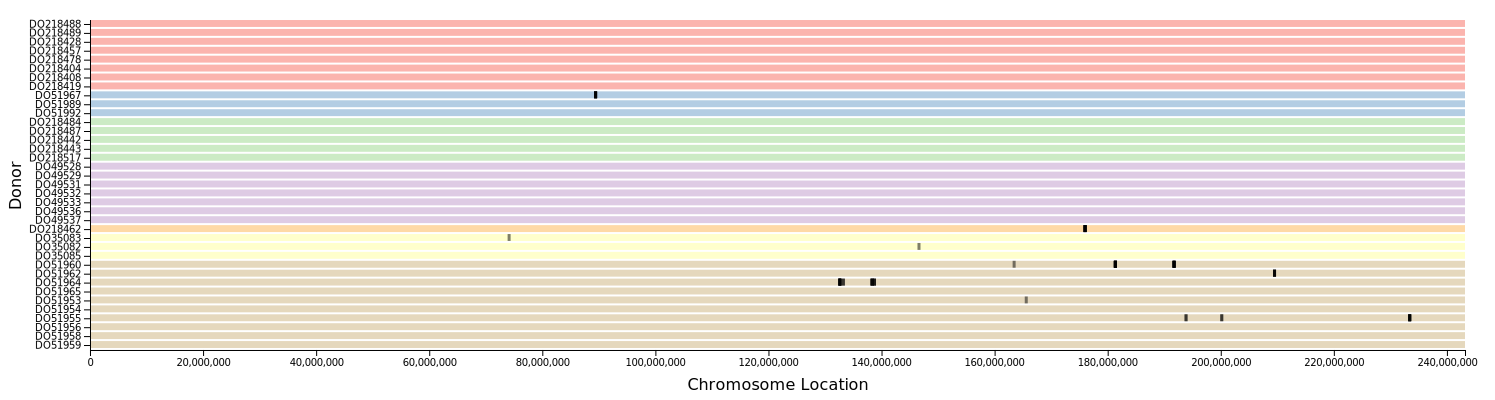
\includegraphics[width=\columnwidth]{figures/kataegis_chr2.pdf}
\end{figure}
\begin{figure}[h!]
    \caption{Rainfall Plot (Chromosome 2)}
    \centering
    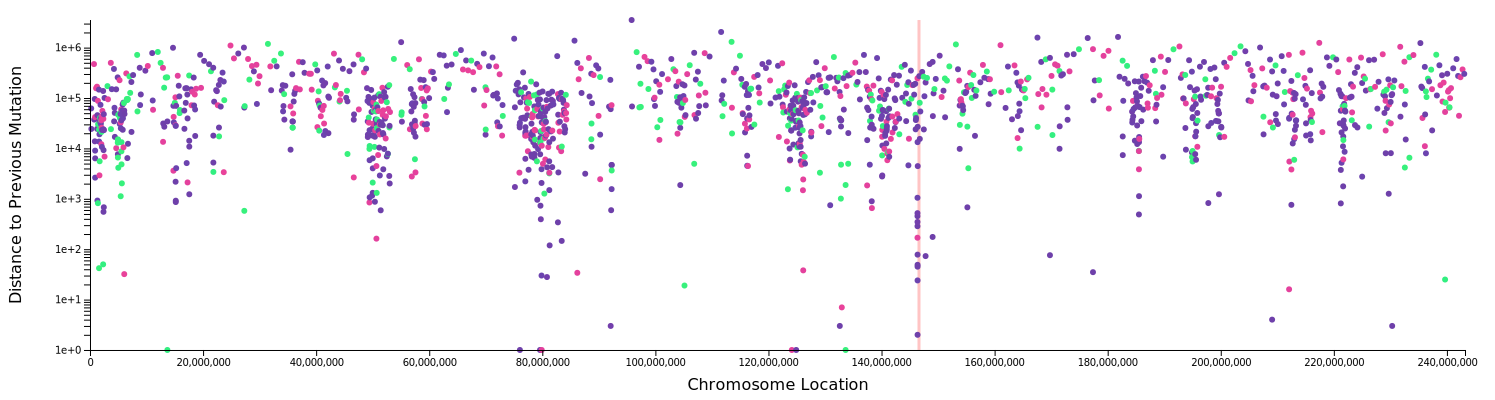
\includegraphics[width=\columnwidth]{figures/rainfall_DO35082_chr2.pdf}
\end{figure}
\begin{figure}[h!]
    \caption{Manhattan Plot (Chromosome 2)}
    \centering
    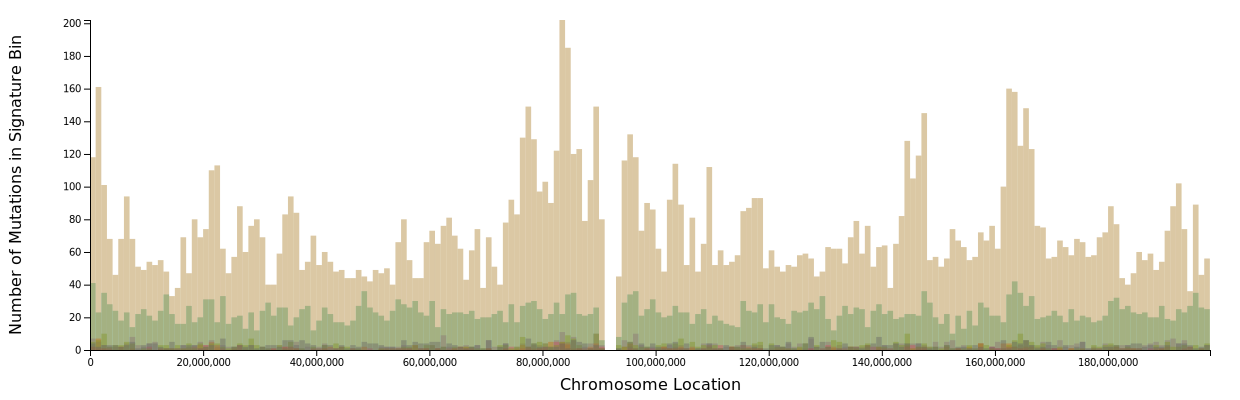
\includegraphics[width=\columnwidth]{figures/manhattan.pdf}
\end{figure}

\end{document}
